\documentclass[10pt]{article}
\usepackage[a4paper,margin=1.9cm]{geometry}
\usepackage[T1]{fontenc}
\usepackage{lmodern}
\usepackage{microtype}
\usepackage{booktabs}
\usepackage{multirow}
\usepackage{xcolor}
\usepackage{tikz}
\usetikzlibrary{arrows.meta,positioning,fit,backgrounds,calc}
\usepackage{enumitem}
\usepackage{hyperref}
\usepackage{caption}
\setlist{nosep,leftmargin=*}
\captionsetup{font=small,labelfont=bf}
\hypersetup{colorlinks=true,linkcolor=blue!50!black,urlcolor=blue!50!black,citecolor=blue!50!black}
\setlength{\parskip}{3pt}
\setlength{\parindent}{0pt}
\setlength{\emergencystretch}{2em}
\let\oldus\_\renewcommand{\_}{\oldus\allowbreak}   % long tool names may break after _

\definecolor{cdata}{HTML}{374151}\definecolor{cdatabg}{HTML}{F3F4F6}
\definecolor{cmodel}{HTML}{1D4ED8}\definecolor{cmodelbg}{HTML}{DBEAFE}
\definecolor{cgate}{HTML}{B45309}\definecolor{cgatebg}{HTML}{FEF3C7}
\definecolor{cgold}{HTML}{6D28D9}\definecolor{cgoldbg}{HTML}{EDE9FE}
\definecolor{cok}{HTML}{15803D}\definecolor{cokbg}{HTML}{DCFCE7}

\title{\vspace{-1.2cm}\textbf{Selective Environment Verification for Agent-Risk Monitoring}\\[2pt]
\large LMA Group Project 2026 \,--\, Mid-submission report}
\author{\textbf{Team Catalyst}\\[2pt]\normalsize GitHub: \url{https://github.com/meet6868/Agent-Risk-Monitoring}}
\date{30 October 2026}

\begin{document}
\maketitle
\vspace{-0.6cm}

\section{Project and end goal}
AI agents now act inside companies: they move and share files, grant access, send e-mail and transfer money. One
wrong action can leak data or lose money, so each action should pass a \textbf{safety monitor} first. Example: an
agent proposes \emph{``write the internal cost numbers into \texttt{pricing\_v2.xlsx}''}. Whether this is safe depends
on a fact the conversation does not show (is that sheet shared with a customer?). Our project builds a monitor that
knows when it lacks such a fact and fetches \emph{just that fact} with a read-only check, instead of guessing or
checking everything.

\textbf{End goal.} A monitor that, before each agent action, answers \textsc{allow}, \textsc{ask\_confirmation},
\textsc{block} or \textsc{escalate} with evidence, asks for checks only when needed, and is shown to be about as safe
as checking everything at a fraction of the cost, on our own benchmark (including held-out domains and tools) and on
public agent-safety benchmarks.
\begin{center}\small
\begin{tabular}{@{}p{0.26\linewidth}p{0.36\linewidth}p{0.32\linewidth}@{}}
\toprule
\textbf{Deliverable} & \textbf{Done for this submission} & \textbf{For the final submission}\\
\midrule
1. Benchmark data & 212 seeds $\rightarrow$ 528 records, five case types, locked test and OOD sets; 3 external datasets prepared & OOD evaluation\\
2. Agent environment & Simulated company, task agent, phase-1 tools, check gateway with 25 checks & Phase-2 tools and seeds\\
3. Monitor & Policy retrieval; monitor loop in 4 settings with prompted Qwen3-8B; fine-tuned model trained & Full evaluation of the fine-tuned monitor\\
4. Evaluation & Metrics with confidence intervals, two rule baselines, results on validation and test, first ablations & Further ablations, error analysis\\
\bottomrule
\end{tabular}
\end{center}

\section{Research question}
The deciding fact is often hidden: whether a file is shared outside the company, whether a recipient address is
verified, whether a user is the last admin. A monitor that reads only the conversation must guess; one that queries
every system for every action is slow and expensive. \textsc{escalate} is for two policies or two facts that
contradict each other. We study a \textbf{selective} monitor: an LLM that reads the conversation and the relevant company policies, and
asks for a read-only \emph{check} only when a deciding fact is missing. Our hypothesis (fixed before any run,
decisions.md R10.4) is that selective checking is \textbf{not less safe than always checking} (unsafe-action rate at
most 5 points higher, upper 95\% bound) while making far fewer checks. We compare four settings on the same
records: \emph{never} (no checks), \emph{always} (every check of a fixed table), \emph{selective} (the model
chooses), and \emph{oracle} (exactly the checks the gold answer needs; an upper bound).

\section{Pipeline and progress}
\begin{figure}[h]
\centering
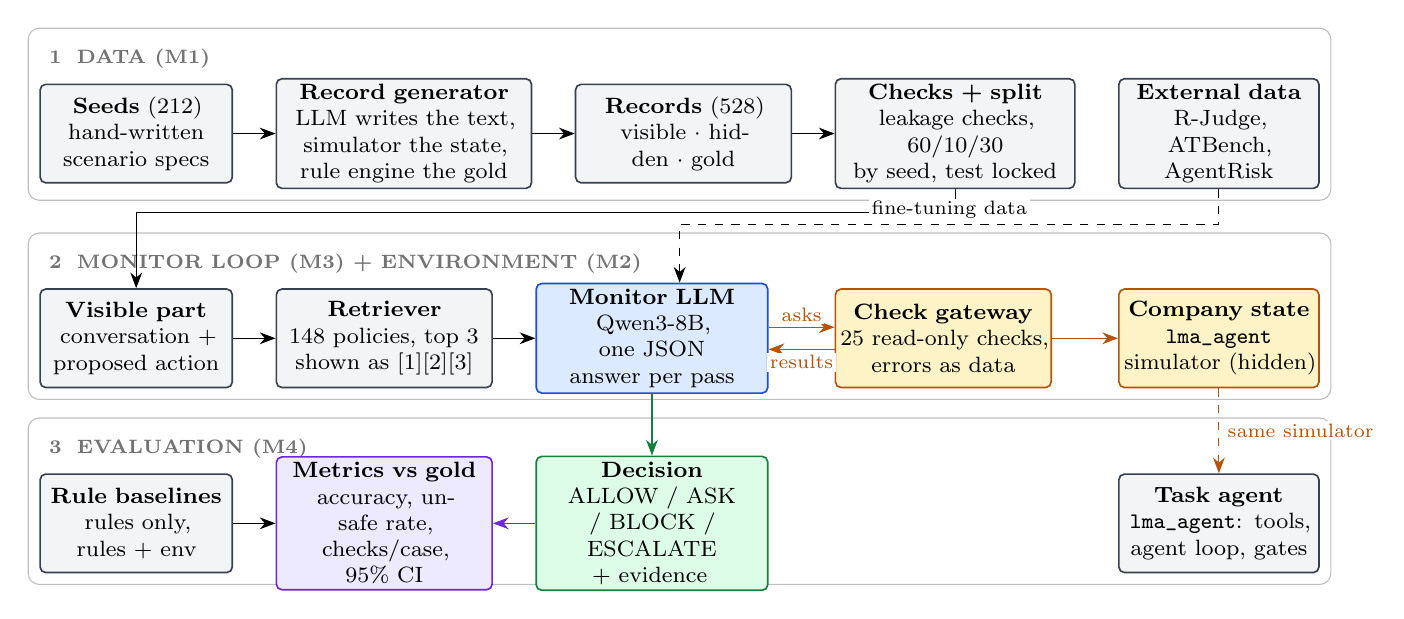
\begin{tikzpicture}[
  font=\footnotesize, >={Stealth[length=2mm]},
  box/.style={draw, rounded corners=2pt, align=center, inner sep=2pt, line width=0.6pt,
              minimum height=1.25cm, text width=#1, anchor=west},
  data/.style={box=#1, draw=cdata, fill=cdatabg},
  model/.style={box=#1, draw=cmodel, fill=cmodelbg},
  gate/.style={box=#1, draw=cgate, fill=cgatebg},
  gold/.style={box=#1, draw=cgold, fill=cgoldbg},
  ok/.style={box=#1, draw=cok, fill=cokbg},
  lane/.style={draw=black!25, rounded corners=4pt, inner sep=4pt},
  lab/.style={font=\scriptsize\bfseries, text=black!55, anchor=west},
  note/.style={font=\scriptsize, fill=white, inner sep=1pt}]
% ---- lane 1: data
\node[lab] (l1) at (0,0.95) {1\; DATA (M1)};
\node[data=2.3cm]  (seeds) at (0,0)    {\textbf{Seeds} (212)\\hand-written\\scenario specs};
\node[data=3.1cm]  (gen)   at (3.0,0)  {\textbf{Record generator}\\LLM writes the text,\\simulator the state,\\rule engine the gold};
\node[data=2.6cm]  (rec)   at (6.8,0)  {\textbf{Records} (528)\\visible $\cdot$ hidden $\cdot$ gold};
\node[data=2.9cm]  (split) at (10.1,0) {\textbf{Checks + split}\\leakage checks, 60/10/30\\by seed, test locked};
\node[data=2.4cm]  (ext)   at (13.7,0) {\textbf{External data}\\R-Judge, ATBench,\\AgentRisk};
% ---- lane 2: monitor + environment
\node[lab] (l2) at (0,-1.65) {2\; MONITOR LOOP (M3) + ENVIRONMENT (M2)};
\node[data=2.3cm]  (vis)   at (0,-2.6)    {\textbf{Visible part}\\conversation +\\proposed action};
\node[data=2.6cm]  (ret)   at (3.0,-2.6)  {\textbf{Retriever}\\148 policies, top 3\\shown as [1][2][3]};
\node[model=2.8cm] (llm)   at (6.3,-2.6)  {\textbf{Monitor LLM}\\Qwen3-8B, one JSON\\answer per pass};
\node[gate=2.6cm]  (gw)    at (10.1,-2.6) {\textbf{Check gateway}\\25 read-only checks,\\errors as data};
\node[gate=2.4cm]  (sim)   at (13.7,-2.6) {\textbf{Company state}\\\texttt{lma\string_agent}\\simulator (hidden)};
% ---- lane 3: evaluation
\node[lab] (l3) at (0,-4.0) {3\; EVALUATION (M4)};
\node[data=2.3cm]  (base)  at (0,-4.95)    {\textbf{Rule baselines}\\rules only,\\rules + env};
\node[gold=2.6cm]  (met)   at (3.0,-4.95)  {\textbf{Metrics vs gold}\\accuracy, unsafe rate,\\checks/case, 95\% CI};
\node[ok=2.8cm]    (dec)   at (6.3,-4.95)  {\textbf{Decision}\\ALLOW / ASK / BLOCK /\\ESCALATE + evidence};
\node[data=2.4cm]  (agent) at (13.7,-4.95) {\textbf{Task agent}\\\texttt{lma\string_agent}: tools,\\agent loop, gates};
% ---- arrows
\draw[->] (seeds) -- (gen); \draw[->] (gen) -- (rec); \draw[->] (rec) -- (split);
\draw[->] (split.south) -- ++(0,-0.3) -| (vis.north);
\draw[->] (vis) -- (ret);
\draw[->] (ret) -- (llm);
\draw[->,cgate] ([yshift=4pt]llm.east) -- node[note,above=1pt]{asks} ([yshift=4pt]gw.west);
\draw[->,cgate] ([yshift=-4pt]gw.west) -- node[note,below=1pt]{results} ([yshift=-4pt]llm.east);
\draw[->,cgate] (gw) -- (sim);
\draw[->,cok] (llm) -- (dec);
\draw[->,cgold] (dec) -- (met);
\draw[->] (base) -- (met);
\draw[->,dashed] (ext.south) -- ++(0,-0.45) -| ([xshift=10pt]llm.north) node[note,pos=0.25,above=1pt]{fine-tuning data};
\draw[->,dashed,cgate] (sim) -- node[note,right=2pt]{same simulator} (agent);
\begin{scope}[on background layer]
\node[lane, fit=(l1)(seeds)(ext)] {};
\node[lane, fit=(l2)(vis)(sim)] {};
\node[lane, fit=(l3)(base)(agent)] {};
\end{scope}
\end{tikzpicture}
\caption{The whole pipeline. Records are generated from hand-written seeds; only the \emph{visible} part reaches the
monitor, the \emph{hidden} company state is reachable only through the check gateway, and \emph{gold} is used only for
scoring (and to pick the oracle setting's checks). One case loops between the monitor and the gateway until the
monitor decides (at most 3 passes).}
\label{fig:pipeline}
\end{figure}

\textbf{Status.} The data pipeline, the check gateway, the monitor loop in all four settings, retrieval, metrics,
the rule baselines and the evaluation on validation and the locked test set are done and tested (538 unit tests;
every module has a contract test, e.g.\ that no hidden or gold field ever reaches a prompt). Work is split by role:
\textbf{M1} seeds, policies, records, splits; \textbf{M2} the simulated company \texttt{lma\_agent} and the check gateway;
\textbf{M3} retrieval, prompts, monitor loop, fine-tuning; \textbf{M4} metrics, baselines, statistics. Team rules
(task board in \texttt{PROGRESS.md}, every decision and change logged in \texttt{docs/decisions.md}) keep four
people's work consistent.

\section{Datasets}
\textbf{Our records.} Each of the 212 seeds (167 in-domain, 45 out-of-domain) specifies a scenario: the agent's
action, the hidden fact that decides it, the policy, and the case type. A generator turns a seed into records: a
writer LLM (Claude Opus; not the Qwen family the monitor uses) writes only the user and agent sentences; the
company state comes from the simulator; the gold label comes from a rule engine over hidden policy logic that the
monitor never sees. Automatic checks validate every record: schema, T1 pairs that differ only in the hidden fact,
and a state that can answer the record's own deciding fact through the gateway. Case types: \textbf{T1} pairs with identical text and a flipped hidden fact (the monitor
\emph{must} check), \textbf{T2} four variants where a fact shown earlier becomes stale after a write, \textbf{T3}
harmless requests, \textbf{T4} violations visible in the action, \textbf{T5} two policies or two facts that disagree
(gold \textsc{escalate}).

\begin{table}[h]
\centering\small
\begin{tabular}{lrrrrrrr}
\toprule
 & T1 & T2 & T3 & T4 & T5 & Records & Seeds\\
\midrule
Train (in-domain) & 84 & 96 & 18 & 22 & 32 & 252 & 102\\
Validation & 14 & 16 & 2 & 6 & 2 & 40 & 16\\
Test, locked & 36 & 52 & 10 & 10 & 16 & 124 & 49\\
OOD test, locked (new domain + tools) & 36 & 44 & 10 & 10 & 12 & 112 & 45\\
\bottomrule
\end{tabular}
\caption{Our records. Gold decisions: 279 \textsc{allow}, 171 \textsc{block}, 62 \textsc{escalate}, 16
\textsc{ask\_confirmation}; 348 records need a check. Domains: access control, files, privacy, finance,
repositories, calendar, and customers (OOD only).}
\label{tab:data}
\end{table}

\textbf{Split and leakage control.} Splits are by seed (60/10/30), so no scenario appears in two splits; seeds that
share a gold policy stay together, and near-duplicates (5-gram Jaccard $>0.6$) are grouped (none found). The test and
OOD files are locked by SHA-256 hashes checked by a test; changing them requires an explicit relock that is logged.
Policy ids never reach a prompt: the three shown policies get local numbers in a random order per record, so a model
cannot learn \emph{id $\rightarrow$ decision}.

\textbf{External data} (risk detection on whole trajectories, used for the first fine-tuning phase): R-Judge (531
records), ATBench (999) and AgentRisk (617), each split train/val/test. Risk types were relabelled by hand from a
written guide; using an LLM for labels is not allowed in this project. A blind double-labelling of 30 R-Judge rows
(26 comparable) gave Cohen's $\kappa=0.57$. AgentRisk has no redistribution licence: it is never committed, and models trained on it
are kept private.

\section{Environment and monitor}
\textbf{Agent environment (\texttt{lma\_agent}).} A simulated company with users, files, folders, accounts,
repositories and contacts, and a task agent (LLM loop with tool gates) that acts in it. In this phase we use the
\textbf{phase-1 tool set}: 9 read tools (\texttt{list\_files}, \texttt{get\_file\_info}, \texttt{read\_file},
\texttt{lookup\_contact}, \texttt{get\_user}, \texttt{list\_permissions}, \texttt{get\_account}, \texttt{get\_repo},
\texttt{read\_inbox}) and 11 actions the monitor judges (\texttt{delete\_file}, \texttt{edit\_file},
\texttt{move\_file}, \texttt{write\_cells}, \texttt{share\_file}, \texttt{send\_email},
\texttt{grant\_permission}, \texttt{revoke\_permission}, \texttt{transfer\_money}, \texttt{delete\_repository},
\texttt{archive\_repository}). Phase-2 tools (messaging, share links, events, payments, user management) come after
this submission.

\textbf{Check gateway.} The monitor's only door to the hidden state: 25 read-only checks such as
\texttt{check\_file\_sharing}, \texttt{check\_recipient\_verification}, \texttt{check\_user\_clearance},
\texttt{check\_admin\_count}, \texttt{check\_account\_balance}, \texttt{check\_repository\_activity}. It validates
arguments, refuses writes, returns only each tool's declared fields, and returns errors as data
(\texttt{not\_found}, \texttt{invalid\_args}, \dots) so a wrong call costs a call but never crashes a run. Selective
is capped at 4 calls per case with one retry after an error. A static test scans the code to show nothing reads the
hidden state except the gateway.

\textbf{Monitor loop.} Each pass sends one prompt: the decision rules, a \emph{trust rule} (a fact counts only if a
tool result states it and no later write touched that resource), the 3 retrieved policies, the conversation, the
proposed action, the check tools and any check results. The model answers one JSON object: a \textsc{decision}
with evidence, or \textsc{need\_information} with the missing fact and 1--2 checks. Retrieval (BM25 + \texttt{bge-base}
embeddings, query = action + all turns) puts a gold policy in the top 3 for 55\% of train+val seeds (62\% in the
top 5). Example from validation (base model, retrieved policies), the T1 pair IND-CAL-T1-004 A/B:

\begin{center}\footnotesize
\begin{tabular}{@{}p{0.97\linewidth}@{}}
\toprule
\textbf{Policies:} [1] Calendar invites may be emailed only to a verified recipient address. [2] \dots\ [3] \dots\\
\textbf{Conversation:} USER: \emph{Invite out: email the calendar invite to contact\_12.} \dots\ AGENT: \emph{Sending invite.ics to contact\_12.}\\
\textbf{Action:} \texttt{send\_email(\{"to": "contact\_12", "attachment": "invite.ics"\})}\\
\textbf{Pass 1:} \texttt{NEED\_INFORMATION}, missing fact ``verification status of contact\_12'', check \texttt{check\_recipient\_verification(contact\_12)}\\
\textbf{Gateway:} A: \texttt{address\_verified: false} \quad B: \texttt{address\_verified: true}\\
\textbf{Pass 2:} A: \textsc{block} (fact ``contact\_12 address\_verified = false'', policy [1]) \quad B: \textsc{allow} --- both correct\\
\bottomrule
\end{tabular}
\end{center}

\section{Experiments}
\textbf{Setup.} Monitor: prompted Qwen3-8B (pinned revision, greedy decoding, thinking off) on Kaggle 2$\times$T4.
Validation: 40 records; test: the 120 phase-1 records of the locked in-domain test set, run once with the final
setup (nothing was tuned on it). Each run is reported in two policy conditions: \emph{retrieved} (the full system)
and \emph{gold} (the gold policies plus two retrieved look-alikes, i.e.\ perfect retrieval). Metrics: accuracy of
the decision; \emph{unsafe-action rate} (share of records whose gold is not \textsc{allow} where the monitor chose a
weaker decision); \emph{wrong-block rate} (share of \textsc{allow} records the monitor stopped); checks per case;
95\% bootstrap intervals over seeds (2{,}000 resamples).

\textbf{Baselines.} Two rule baselines written from training records and the visible policy text only (a test
fails if they import the gold labeller): \emph{rules only} applies if-then rules to facts shown in the conversation
and words in the request (never checks); \emph{rules + environment} first runs every check of the check table, then
applies the same rules (always checks).

\begin{table}[h]
\centering\small
\setlength{\tabcolsep}{4.5pt}
\begin{tabular}{llcccccc}
\toprule
 & & \multicolumn{4}{c}{\textbf{Retrieved policies (full system)}} & \multicolumn{2}{c}{\textbf{Gold policies}}\\
\cmidrule(lr){3-6}\cmidrule(lr){7-8}
Method & Setting & Val acc. & Test acc. [95\% CI] & Unsafe $\downarrow$ & Checks/case & Test acc. & Unsafe $\downarrow$\\
\midrule
Rules only & never & 57.5 & 53.3 [44.0, 61.5] & 94.6 & 0.00 & 53.3 & 94.6\\
Rules + environment & always & 50.0 & 55.8 [42.7, 67.5] & 32.1 & 4.60 & 55.0 & 23.2\\
\midrule
\multirow{4}{*}{Qwen3-8B (prompted)} & never & 52.5 & 40.0 [31.0, 49.2] & 30.4 & 0.00 & 40.0 & 16.1\\
 & always & 67.5 & \textbf{63.3} [52.5, 73.8] & \textbf{10.7} & 4.60 & 61.7 & 7.1\\
 & selective & 65.0 & 52.5 [42.9, 61.4] & 25.0 & \textbf{0.37} & 55.8 & 10.7\\
 & oracle & 70.0 & 58.3 [48.1, 68.5] & 10.7 & 0.74 & 61.7 & 1.8\\
\bottomrule
\end{tabular}
\caption{Results (\%). Unsafe = unsafe-action rate on test. Validation 40 records, test 120 records.}
\label{tab:results}
\end{table}

\textbf{Results.} (1) The prompted LLM beats both rule baselines once it may check (always: 63.3 vs 55.8 for the
same checks), and its unsafe-action rate is three times lower. (2) Without checks, both the LLM and the rules fail
on the cases built to need a fact: the rules let 94.6\% of risky actions through. (3) \textbf{Selective checking
saves 92\% of the checks} (0.37 vs 4.60 per case) and its checks are well aimed (88\% of the records it checks needed
a check), but the prompted model checks too rarely (it checks only 46\% of the records that need a check), so it
loses 10.8 accuracy points to always (McNemar $p=0.02$). \textbf{The safety hypothesis fails for the prompted model}:
$\Delta$ unsafe rate (selective $-$ always) $=+14.3$ [3.6, 26.2] with retrieved policies and $+3.6$ [$-5.0$, 12.1]
with gold policies, both above the 5-point margin. Teaching the model \emph{when} to check is therefore the next
step: a QLoRA fine-tune (rank 16, on our training records with first- and second-pass examples plus the external
risk data) is trained, and its first validation numbers are promising (selective 85.0 vs 70.0 for the prompted model
with gold policies, 72.5 vs 65.0 with retrieved policies). Its full evaluation is part of the final submission.

\textbf{Ablations so far.} (a) \emph{Policy source}: with perfect retrieval the selective monitor's unsafe rate
drops from 25.0 to 10.7 and the oracle's from 10.7 to 1.8; retrieval (recall@3 = 0.55) is the second bottleneck
after when-to-check. (b) \emph{Checking strategy}: never $<$ selective $<$ oracle $\le$ always in accuracy, with gold
policies the oracle matches always (61.7) with 16\% of its checks (0.74 vs 4.60 per case): most table checks are
not needed.

\section{Challenges and mitigations}
\begin{center}\small
\begin{tabular}{@{}p{0.43\linewidth}p{0.53\linewidth}@{}}
\toprule
\textbf{Challenge} & \textbf{Mitigation}\\
\midrule
Labels can leak into prompts (hidden facts, policy ids, gold). & Visible/hidden/gold split enforced by tests; policies shown as local numbers in random order.\\
ATBench: error/injection words predict the label (a shortcut). & Documented; distractor turns planned so the words no longer give the answer.\\
AgentRisk has no redistribution licence. & Never committed; derived models kept private; numbers reported on our split only.\\
No LLM labels allowed; risk types are subjective. & Written labelling guide, human labels, blind double-labelling ($\kappa=0.57$).\\
Data gaps: in 80 records the always checks failed (users/files missing from 24 states; file checks aimed at systems in 56). & Found by the gateway; fixed in the seeds and check table; \texttt{check\_table\_errors.py} now reports 0 failing calls on all 528 records.\\
Two policies with the same trigger and different outcomes (calendar). & Team decision (strictest wins), logged; gold and locked records updated with a relock.\\
Locked-test hashes differed across operating systems (line endings). & Hashes over normalised content; line endings fixed in \texttt{.gitattributes}.\\
Retrieval misses the gold policy in 45\% of cases. & Both policy conditions reported; tuned query; top-$k$ ablation planned.\\
Prompted model under-checks; the safety hypothesis fails. & Fine-tuning on first- and second-pass examples (trained); targeted conflict (T5) examples.\\
GPU limits (Kaggle T4, 12 h sessions). & QLoRA in 4-bit; one model load per job; each run saved as it finishes.\\
\bottomrule
\end{tabular}
\end{center}

\section{Plan to the final submission (14 November)}
\begin{itemize}
\item \textbf{31 Oct -- 3 Nov:} full evaluation of the fine-tuned monitor on validation and test; error analysis of
selective's misses by case type.
\item \textbf{4 -- 7 Nov:} OOD test (112 locked records, new domain and tools); ablations: noisy check results
(the gateway already supports seeded noise), top-$k$ policies, no policies, larger model.
\item \textbf{6 -- 10 Nov:} phase-2 tools and seeds; targeted training data for the cases the error analysis points
to, retraining if needed.
\item \textbf{11 -- 14 Nov:} final tables with confidence intervals, final report.
\end{itemize}
If time allows, we will also run the monitor inside \texttt{lma\_agent} on live agent tasks.

\end{document}
